\documentclass[11pt]{article}

\usepackage{booktabs}
\usepackage{homeworkpkg}
\usepackage{enumitem}
\usepackage{xcolor,listings}
\usepackage{caption}
\usepackage{multirow}
\usepackage{multicol}

\graphicspath{ {images/} }

%% Local Macros and packages: add any of your own definitions here.

\begin{document}

% Homework number, your name and NetID, and optionally, the names/NetIDs of anyone you collaborated with. If you did not collaborate with anybody, leave the last parameter empty.
\homework
    {4}
    {Nestor Alejandro Bermudez Sarmiento (nab6)}
    {}


\section*{Introduction}

This report covers the implementation details and results of two different classification methods applied in four different data sets. The first method explored is Decision Trees: a tree data structure that encodes every possible outcome of a decision. There are many ways to construct such tree. Decision Trees are quite popular because their performance is decent but more importantly, they are easily interpretable by humans.\\

As in any classification method, over-fitting is a problem. When working with Decision Trees one way to alleviate this problem is to reduce the depth of the tree or set minimum sizes required to split a node or of the split branch itself. These are the hyper-parameters of the classifier and in the following section I'll provide the values used for the different data sets.\\

The second classification method covered in this report is an ensemble method called Random Forest first developed by Tim Kan Ho in 1995 and later extended by Leo Brieman. Random Forest provide the advantage of 'smoothing out' the error and over-fitting present in normal Decision Trees based on the idea that as the number of trees increase, the chances of over-fitting the same values multiple times decreases. \\

The hyper-parameters for Random Forest include the number of trees, how much data bagging should be performed, what percentage of the features should be considered for every tree and the hyper-parameters for the Decision Tree itself. It is common to not limit the depth of the tree when using Random Forest because the randomness and the number of trees takes care of the over-fitting problem in this case. I will explore different configurations of hyper-parameters to confirm this.

\section*{Implementation details}

The classification methods have been implemented using Python and nothing more than the features available in the standard library of the language in order to better grasp the details of the algorithms. I decided to use Python 3 over Python 2 because of the introduction of \textit{lru\_cache} which provides an easy way to do some basic caching and enhance performance.\\

The code follows a very object oriented structure. You will find classes that handle reading the content from the file and creating an internal representation; a \textbf{Dataset} class that wraps the reader class and provides helper methods to split the data by attribute or class and get info about the examples in it; calculate the Gini index; get the metrics given a confusion matrix and, print out the results.\\

The main programs, \textbf{DecisionTree.py} and \textbf{RandomForest.py}, take on multiple flags that change the behavior. When run without flags it uses the parameters mentioned in the next section and output simply the confusion matrix. They support flags to calculate and display the different metrics per class, do a grid search to find the appropriate parameters and, re-sample the training data.\\

The code makes use of the \textit{multiprocessing} package to run some code in parallel. In the case of the Decision Tree, the branch construction happens in parallel for some of the data sets and, in the case of Random Forest, the trees are built in parallel.

\subsection*{Decision Tree}

\subsubsection*{Parameter choices}

As mentioned in the Introduction, the hyper-parameters for Decision Tree that I used are: depth, minimum split size (\textit{minsplit}) and minimum leaf size (\textit{minleaf}). The \textit{minleaf} parameter indicates that if, after splitting, the node would contain less than the given amount it should be classify test examples based on the most frequent sibling branch. The following table summarizes the values chosen for every data set.

\begin{center}
\begin{tabular}{cc|r|r|r|l}
\cline{3-5}
& & \multicolumn{3}{ c| }{Hyper-parameters} \\ \cline{3-5}
& & Depth & Minsplit & Minleaf  \\ \cline{1-5}
\multicolumn{1}{ |c  }{\multirow{4}{*}{Data set} } &
\multicolumn{1}{ |l| }{Balance scale} & -1 & 2 & 1   \\ \cline{2-5}
\multicolumn{1}{ |c  }{}                        &
\multicolumn{1}{ |l| }{Led} & 5 & 1 & 1   \\ \cline{2-5}
\multicolumn{1}{ |c  }{}                        &
\multicolumn{1}{ |l| }{Nursery} & -1* & 1 & -1*   \\ \cline{2-5}
\multicolumn{1}{ |c  }{}                        &
\multicolumn{1}{ |l| }{Synthetic Social} & 13 & 66 & 1  \\ \cline{1-5}
\end{tabular}
\captionof{table}{Hyper-parameters for every data set evaluated. The value -1 means unbounded.}
\end{center}

The values for the parameters were found using Grid Search with increments of 1. In the case of the Nursery data set, the search was interrupted early after seeing that the result with default parameters had a very high accuracy and the parameters so far did not improve it. For all the data sets, the search would be stopped if the execution time took more than 180 seconds. \\

An additional parameter used is a boolean flag that decides whether to use parallelism to build the tree or not. This flag is \textbf{False} for all the data sets except Synthetic Social. The reason for this is that the first three data sets are small enough that the parallelism actually hurts performance because of the hidden cost of shared memory and locks. In the case of Synthetic Social this added cost is outweighed by the benefit of building the branches in parallel.

\subsection*{Random Forest}

\subsubsection*{Parameter choices}

On top of the hyper-parameters for the Decision Tree I have three new ones for Random Forest: number of trees (\textit{size}), data bagging (\textit{dbag \%}) and feature bagging (\textit{fbag \%}). The following table summarizes all the chosen values.

\begin{center}
\begin{tabular}{cc|r|r|r|r|r|r|l}
\cline{3-8}
& & \multicolumn{6}{ c| }{Hyper-parameters} \\ \cline{3-8}
& & Depth & Minsplit & Minleaf & Size & DBag \% & FBag \%  \\ \cline{1-8}
\multicolumn{1}{ |c  }{\multirow{4}{*}{Data set} } &
\multicolumn{1}{ |l| }{Balance scale} & -1 & 3 & 8 & 41 & 60 & 25  \\ \cline{2-8}
\multicolumn{1}{ |c  }{}                        &
\multicolumn{1}{ |l| }{Led} & -1 & 1 & 1 & 51 & 67 & 100   \\ \cline{2-8}
\multicolumn{1}{ |c  }{}                        &
\multicolumn{1}{ |l| }{Nursery} & -1 & 1 & -1 & 101 & 70 & 90   \\ \cline{2-8}
\multicolumn{1}{ |c  }{}                        &
\multicolumn{1}{ |l| }{Synthetic Social} & -1 & 3 & 1 & 70 & 96.50 & 3.16  \\ \cline{1-8}
\end{tabular}
\captionof{table}{Hyper-parameters for every data set evaluated}
\end{center}

For all the data sets except Synthetic Social the values where chosen using Grid Search on the size, dbag and fbag \%. The values were constantly incremented by 1 on every case and the search would skip a dimension once the execution time exceeded 180 seconds. This was a valid argument because the execution time increases as the value of each of those parameters increase. The other three parameters (depth, minsplit and minleaf) were chosen by first trying the values from the single Decision Tree analysis; if those didn't work I tried unbounded values; if even after that the accuracy would not improve I did local grid search on those two (with the already fixed values for the other 3 parameters). \\

For the Synthetic Social data set I tried to use Grid Search but it proven too impractical, the accuracies gotten were really inconsistent. Finally I decided to use a random search on the dbag and fbag \% parameters using a fixed size (10). For the parameter values that passed a threshold (60\% accuracy) I would then run 10 iterations and get the mean, min and max accuracy obtained from those 10 iterations. Finally I chose the values that gave a high accuracy and low distance between the min and max accuracies. \\
Once I fixed the dbag and fbag parameters I tried different sizes. Overall, as the size increased the accuracy did too so I decided to take a size that was large enough give a good accuracy and still run under the time constraint imposed (180 seconds).

\pagebreak
\section*{Results}

\subsection*{Decision Tree}
\subsubsection*{Balance Scale Data set}

Lets first look at the metrics for the test data set. 

\begin{center}
\begin{tabular}{cc|r|r|r|}
\cline{3-5}
& & \multicolumn{3}{ c| }{Predicted class} \\ \cline{3-5}
& & 1 & 2 & 3  \\ \cline{1-5}
\multicolumn{1}{ |c  }{\multirow{3}{*}{Expected class} } &
\multicolumn{1}{ |r| }{1} & 0 & 14 & 8    \\ \cline{2-5}
\multicolumn{1}{ |c  }{}                        &
\multicolumn{1}{ |r| }{2} & 2 & 81 & 19    \\ \cline{2-5}
\multicolumn{1}{ |c  }{}                        &
\multicolumn{1}{ |c| }{3} & 12 & 16 & 73  \\ \cline{1-5}
\end{tabular}
\captionof{table}{Confusion matrix for test data.}
\end{center}

Now, the metrics calculated from the confusion matrix.
\begin{center}
\begin{tabular}{c|r|r|r|}
\cline{2-4}
& \multicolumn{3}{ c| }{Class} \\ \cline{2-4}
& 1 & 2 & 3  \\ \cline{1-4}
\multicolumn{1}{ |l| }{Accuracy} & 84.0 & 77.33 & 75.56    \\ \cline{1-4}
\multicolumn{1}{ |l| }{F-1 Score} & 0.00 & 76.06 & 71.64    \\ \cline{1-4}
\multicolumn{1}{ |l| }{F-0.5 Score} & 0.00 & 78.03 & 72.42    \\ \cline{1-4}
\multicolumn{1}{ |l| }{F-2 Score} & 0.00 & 74.18 & 72.85    \\ \cline{1-4}
\multicolumn{1}{ |l| }{Precision} & 0.00 & 72.97 & 73.00    \\ \cline{1-4}
\multicolumn{1}{ |l| }{Recall} & 0.00 & 79.41 & 72.28    \\ \cline{1-4}
\multicolumn{1}{ |l| }{Accuracy} & 93.1 & 75.61 & 78.23    \\ \cline{1-4}
\end{tabular}
\captionof{table}{Metrics (percentages) per class for test data set.}
\end{center}

Overall accuracy: \textbf{68.44\%}\\

Now the results of evaluating the model using the training data set.

\begin{center}
\begin{tabular}{cc|r|r|r|}
\cline{3-5}
& & \multicolumn{3}{ c| }{Predicted class} \\ \cline{3-5}
& & 1 & 2 & 3  \\ \cline{1-5}
\multicolumn{1}{ |c  }{\multirow{3}{*}{Expected class} } &
\multicolumn{1}{ |r| }{1} & 8 & 7 & 12    \\ \cline{2-5}
\multicolumn{1}{ |c  }{}                        &
\multicolumn{1}{ |r| }{2} & 4 & 166 & 16    \\ \cline{2-5}
\multicolumn{1}{ |c  }{}                        &
\multicolumn{1}{ |c| }{3} & 2 & 15 & 170  \\ \cline{1-5}
\end{tabular}
\captionof{table}{Confusion matrix for train data.}
\end{center}

And the metrics for the training set confusion matrix.

\begin{center}
\begin{tabular}{c|r|r|r|}
\cline{2-4}
& \multicolumn{3}{ c| }{Class} \\ \cline{2-4}
& 1 & 2 & 3  \\ \cline{1-4}
\multicolumn{1}{ |l| }{Accuracy} & 93.75 & 89.50 & 88.75    \\ \cline{1-4}
\multicolumn{1}{ |l| }{F-1 Score} & 39.02 & 88.77 & 88.31    \\ \cline{1-4}
\multicolumn{1}{ |l| }{F-0.5 Score} & 32.79 & 89.06 & 89.85    \\ \cline{1-4}
\multicolumn{1}{ |l| }{F-2 Score} & 48.19 & 88.49 & 86.82    \\ \cline{1-4}
\multicolumn{1}{ |l| }{Precision} & 57.14 & 88.30 & 85.86    \\ \cline{1-4}
\multicolumn{1}{ |l| }{Recall} & 29.63 & 89.25 & 90.91    \\ \cline{1-4}
\multicolumn{1}{ |l| }{Accuracy} & 98.39 & 89.72 & 86.85    \\ \cline{1-4}
\end{tabular}
\captionof{table}{Metrics (percentages) per class for training data set.}
\end{center}

Overall accuracy: \textbf{86\%}

\pagebreak
\subsubsection*{LED Data set}

Measurements for the evaluation using the test data.

\begin{center}
\begin{tabular}{cc|r|r|r|}
\cline{3-4}
& & \multicolumn{2}{ c| }{Predicted class} \\ \cline{3-4}
& & 1 & 2  \\ \cline{1-4}
\multicolumn{1}{ |c  }{\multirow{2}{*}{Expected class} } &
\multicolumn{1}{ |r| }{1} & 269 & 82    \\ \cline{2-4}
\multicolumn{1}{ |c  }{}                        &
\multicolumn{1}{ |r| }{2} & 80 & 703  \\ \cline{1-4}
\end{tabular}
\captionof{table}{Confusion matrix for test data.}
\end{center}

Per class metrics:
\begin{center}
\begin{tabular}{c|r|r|r|}
\cline{2-3}
& \multicolumn{2}{ c| }{Class} \\ \cline{2-3}
& 1 & 2  \\ \cline{1-3}
\multicolumn{1}{ |l| }{Accuracy} & 85.71 & 85.71    \\ \cline{1-3}
\multicolumn{1}{ |l| }{F-1 Score} & 76.86 & 89.67    \\ \cline{1-3}
\multicolumn{1}{ |l| }{F-0.5 Score} & 76.73 & 89.74    \\ \cline{1-3}
\multicolumn{1}{ |l| }{F-2 Score} & 76.99 & 89.6    \\ \cline{1-3}
\multicolumn{1}{ |l| }{Precision} & 77.08 & 89.55   \\ \cline{1-3}
\multicolumn{1}{ |l| }{Recall} & 76.64 & 89.78    \\ \cline{1-3}
\multicolumn{1}{ |l| }{Accuracy} & 89.78 & 76.64    \\ \cline{1-3}
\end{tabular}
\captionof{table}{Metrics (percentages) per class for training data set.}
\end{center}

Overall accuracy: \textbf{85.71\%}\\

Measurements when evaluating the classifier with the training data.

\begin{center}
\begin{tabular}{cc|r|r|r|}
\cline{3-4}
& & \multicolumn{2}{ c| }{Predicted class} \\ \cline{3-4}
& & 1 & 2  \\ \cline{1-4}
\multicolumn{1}{ |c  }{\multirow{2}{*}{Expected class} } &
\multicolumn{1}{ |r| }{1} & 483 & 155    \\ \cline{2-4}
\multicolumn{1}{ |c  }{}                        &
\multicolumn{1}{ |r| }{2} & 158 & 1291  \\ \cline{1-4}
\end{tabular}
\captionof{table}{Confusion matrix for train data.}
\end{center}

Per class metrics:
\begin{center}
\begin{tabular}{c|r|r|r|}
\cline{2-3}
& \multicolumn{2}{ c| }{Class} \\ \cline{2-3}
& 1 & 2  \\ \cline{1-3}
\multicolumn{1}{ |l| }{Accuracy} & 85.00 & 85.00    \\ \cline{1-3}
\multicolumn{1}{ |l| }{F-1 Score} & 75.53 & 89.19    \\ \cline{1-3}
\multicolumn{1}{ |l| }{F-0.5 Score} & 75.63 & 89.13    \\ \cline{1-3}
\multicolumn{1}{ |l| }{F-2 Score} & 75.42 & 89.24    \\ \cline{1-3}
\multicolumn{1}{ |l| }{Precision} & 75.35 & 89.28   \\ \cline{1-3}
\multicolumn{1}{ |l| }{Recall} & 75.71 & 89.10    \\ \cline{1-3}
\multicolumn{1}{ |l| }{Accuracy} & 89.10 & 75.71    \\ \cline{1-3}
\end{tabular}
\captionof{table}{Metrics (percentages) per class for training data set.}
\end{center}

Overall accuracy: \textbf{85\%}\\

\pagebreak
\subsubsection*{Nursery Data set}

Measurements when evaluating the classifier with the test data.

\begin{center}
\begin{tabular}{cc|r|r|r|r|r|r|}
\cline{3-7}
& & \multicolumn{5}{ c| }{Predicted class} \\ \cline{3-7}
& & 1 & 2 & 3 & 4 & 5 \\ \cline{1-7}
\multicolumn{1}{ |c  }{\multirow{5}{*}{Expected class} } &
\multicolumn{1}{ |r| }{1} & 1539 & 41 & 16 & 0 & 0    \\ \cline{2-7}
\multicolumn{1}{ |c  }{}                        &
\multicolumn{1}{ |r| }{2} & 30 & 95 & 0 & 0 & 3    \\ \cline{2-7}
\multicolumn{1}{ |c  }{}                        &
\multicolumn{1}{ |r| }{3} & 34 & 0 & 1502 & 0 & 0    \\ \cline{2-7}
\multicolumn{1}{ |c  }{}                        &
\multicolumn{1}{ |r| }{4} & 0 & 0 & 0 & 1605 & 0    \\ \cline{2-7}
\multicolumn{1}{ |c  }{}                        &
\multicolumn{1}{ |r| }{5} & 0 & 0 & 0 & 0 &0  \\ \cline{1-7}
\end{tabular}
\captionof{table}{Confusion matrix for test data.}
\end{center}

Per class metrics:
\begin{center}
\begin{tabular}{c|r|r|r|r|r|}
\cline{2-6}
& \multicolumn{5}{ c| }{Class} \\ \cline{2-6}
& 1 & 2 & 3 & 4 & 5  \\ \cline{1-6}
\multicolumn{1}{ |l| }{Accuracy} & 97.49 & 98.42 & 99.01 & 100.0 & 99.94   \\ \cline{1-6}
\multicolumn{1}{ |l| }{F-1 Score} & 96.18 & 71.16 & 98.43 & 100.0 & 0.00    \\ \cline{1-6}
\multicolumn{1}{ |l| }{F-0.5 Score} &  96.26 & 72.3 & 98.16 & 100.0 & 0.00   \\ \cline{1-6}
\multicolumn{1}{ |l| }{F-2 Score} &  96.11 & 70.06 & 98.70 & 100.0 & 0.00    \\ \cline{1-6}
\multicolumn{1}{ |l| }{Precision} &  96.06 & 69.34 & 98.88 & 100.0 & 0.00   \\ \cline{1-6}
\multicolumn{1}{ |l| }{Recall} &  96.3 & 73.08 & 97.98 & 100.0 & 0.00   \\ \cline{1-6}
\multicolumn{1}{ |l| }{Accuracy} &  98.07 & 99.11 & 99.49 & 100.0 & 99.94    \\ \cline{1-6}
\end{tabular}
\captionof{table}{Metrics (percentages) per class for test data set.}
\end{center}

Overall accuracy: \textbf{97.43\%}\\

Measurements when evaluating the model on the training data set.
\begin{center}
\begin{tabular}{cc|r|r|r|r|r|r|}
\cline{3-7}
& & \multicolumn{5}{ c| }{Predicted class} \\ \cline{3-7}
& & 1 & 2 & 3 & 4 & 5 \\ \cline{1-7}
\multicolumn{1}{ |c  }{\multirow{5}{*}{Expected class} } &
\multicolumn{1}{ |r| }{1} & 2670 & 0 & 0 & 0 & 0    \\ \cline{2-7}
\multicolumn{1}{ |c  }{}                        &
\multicolumn{1}{ |r| }{2} & 0 & 198 & 0 & 0 & 0    \\ \cline{2-7}
\multicolumn{1}{ |c  }{}                        &
\multicolumn{1}{ |r| }{3} & 0 & 0 & 2508 & 0 & 0    \\ \cline{2-7}
\multicolumn{1}{ |c  }{}                        &
\multicolumn{1}{ |r| }{4} & 0 & 0 & 0 & 2715 & 0    \\ \cline{2-7}
\multicolumn{1}{ |c  }{}                        &
\multicolumn{1}{ |r| }{5} & 0 & 0 & 0 & 0 &2  \\ \cline{1-7}
\end{tabular}
\captionof{table}{Confusion matrix for train data.}
\end{center}

Per class metrics:
\begin{center}
\begin{tabular}{c|r|r|r|r|r|}
\cline{2-6}
& \multicolumn{5}{ c| }{Class} \\ \cline{2-6}
& 1 & 2 & 3 & 4 & 5  \\ \cline{1-6}
\multicolumn{1}{ |l| }{Accuracy} & 100.0 & 100.0 & 100.0 & 100.0 & 100.0   \\ \cline{1-6}
\multicolumn{1}{ |l| }{F-1 Score}  & 100.0 & 100.0 & 100.0 & 100.0 & 100.0   \\ \cline{1-6}
\multicolumn{1}{ |l| }{F-0.5 Score} & 100.0 & 100.0 & 100.0 & 100.0 & 100.0   \\ \cline{1-6}
\multicolumn{1}{ |l| }{F-2 Score} & 100.0 & 100.0 & 100.0 & 100.0 & 100.0   \\ \cline{1-6}
\multicolumn{1}{ |l| }{Precision} & 100.0 & 100.0 & 100.0 & 100.0 & 100.0   \\ \cline{1-6}
\multicolumn{1}{ |l| }{Recall} & 100.0 & 100.0 & 100.0 & 100.0 & 100.0   \\ \cline{1-6}
\multicolumn{1}{ |l| }{Accuracy} & 100.0 & 100.0 & 100.0 & 100.0 & 100.0   \\ \cline{1-6}
\end{tabular}
\captionof{table}{Metrics (percentages) per class for training data set.}
\end{center}

Overall accuracy: \textbf{100\%}

\pagebreak
\subsubsection*{Synthetic Social Data set}

Measurements when evaluating the classifier with the test data.

\begin{center}
\begin{tabular}{cc|r|r|r|r|r|}
\cline{3-6}
& & \multicolumn{4}{ c| }{Predicted class} \\ \cline{3-6}
& & 1 & 2 & 3 & 4 \\ \cline{1-6}
\multicolumn{1}{ |c  }{\multirow{4}{*}{Expected class} } &
\multicolumn{1}{ |r| }{1} & 117 & 37 & 74 & 40    \\ \cline{2-6}
\multicolumn{1}{ |c  }{}                        &
\multicolumn{1}{ |r| }{2} & 23 & 111 & 55 & 56    \\ \cline{2-6}
\multicolumn{1}{ |c  }{}                        &
\multicolumn{1}{ |r| }{3} & 33 & 39 & 139 & 21    \\ \cline{2-6}
\multicolumn{1}{ |c  }{}                        &
\multicolumn{1}{ |r| }{4} & 54 & 59 & 17 & 125  \\ \cline{1-6}
\end{tabular}
\captionof{table}{Confusion matrix for test data.}
\end{center}

Per class metrics:
\begin{center}
\begin{tabular}{c|r|r|r|r|}
\cline{2-5}
& \multicolumn{4}{ c| }{Class} \\ \cline{2-5}
& 1 & 2 & 3 & 4  \\ \cline{1-5}
\multicolumn{1}{ |l| }{Accuracy} & 73.9 & 73.1 & 76.1 &75.3   \\ \cline{1-5}
\multicolumn{1}{ |l| }{F-1 Score} & 47.27 & 45.21 & 53.77 & 50.30   \\ \cline{1-5}
\multicolumn{1}{ |l| }{F-0.5 Score} & 45.03 & 45.27 & 57.30 & 49.52   \\ \cline{1-5}
\multicolumn{1}{ |l| }{F-2 Score} & 49.74 & 45.16 & 50.66 &51.10   \\ \cline{1-5}
\multicolumn{1}{ |l| }{Precision} & 51.54 & 45.12 & 48.77 & 51.65   \\ \cline{1-5}
\multicolumn{1}{ |l| }{Recall} & 43.66 & 45.31 & 59.91 & 49.02   \\ \cline{1-5}
\multicolumn{1}{ |l| }{Accuracy} & 84.97 & 82.12 & 80.99 & 84.30   \\ \cline{1-5}
\end{tabular}
\captionof{table}{Metrics (percentages) per class for test data set.}
\end{center}

Overall accuracy: \textbf{49.2\%}\\

Measurements when evaluating the model on the training data set.

\begin{center}
\begin{tabular}{cc|r|r|r|r|r|}
\cline{3-6}
& & \multicolumn{4}{ c| }{Predicted class} \\ \cline{3-6}
& & 1 & 2 & 3 & 4 \\ \cline{1-6}
\multicolumn{1}{ |c  }{\multirow{4}{*}{Expected class} } &
\multicolumn{1}{ |r| }{1} & 370 & 87 & 170 & 105    \\ \cline{2-6}
\multicolumn{1}{ |c  }{}                        &
\multicolumn{1}{ |r| }{2} & 65 & 428 & 160 & 102    \\ \cline{2-6}
\multicolumn{1}{ |c  }{}                        &
\multicolumn{1}{ |r| }{3} & 100 & 149 & 479 & 40    \\ \cline{2-6}
\multicolumn{1}{ |c  }{}                        &
\multicolumn{1}{ |r| }{4} & 130 & 151 & 34 & 430  \\ \cline{1-6}
\end{tabular}
\captionof{table}{Confusion matrix for training data.}
\end{center}

Per class metrics:
\begin{center}
\begin{tabular}{c|r|r|r|r|}
\cline{2-5}
& \multicolumn{4}{ c| }{Class} \\ \cline{2-5}
& 1 & 2 & 3 & 4  \\ \cline{1-5}
\multicolumn{1}{ |l| }{Accuracy} & 78.1 & 76.2 & 78.23 & 81.27   \\ \cline{1-5}
\multicolumn{1}{ |l| }{F-1 Score} & 52.97 & 54.52 & 59.47 & 60.48   \\ \cline{1-5}
\multicolumn{1}{ |l| }{F-0.5 Score} & 51.49 & 55.8 & 61.17 & 58.79   \\ \cline{1-5}
\multicolumn{1}{ |l| }{F-2 Score} & 54.54 & 53.3 & 57.85 & 62.26   \\ \cline{1-5}
\multicolumn{1}{ |l| }{Precision} & 55.64 & 53.53 & 56.82 & 63.52   \\ \cline{1-5}
\multicolumn{1}{ |l| }{Recall} & 50.55 & 56.69 & 62.37 & 57.72   \\ \cline{1-5}
\multicolumn{1}{ |l| }{Accuracy} & 86.99 & 82.76 & 83.69 & 89.05   \\ \cline{1-5}
\end{tabular}
\captionof{table}{Metrics (percentages) per class for training data set.}
\end{center}

Overall accuracy: \textbf{56.9\%}\\



\pagebreak
\subsection*{Random Forest}
\subsubsection*{Balance Scale Data set}

Lets first look at the metrics for the test data set. 

\begin{center}
\begin{tabular}{cc|r|r|r|}
\cline{3-5}
& & \multicolumn{3}{ c| }{Predicted class} \\ \cline{3-5}
& & 1 & 2 & 3  \\ \cline{1-5}
\multicolumn{1}{ |c  }{\multirow{3}{*}{Expected class} } &
\multicolumn{1}{ |r| }{1} & 0 & 10 & 12    \\ \cline{2-5}
\multicolumn{1}{ |c  }{}                        &
\multicolumn{1}{ |r| }{2} & 0 & 93 & 9    \\ \cline{2-5}
\multicolumn{1}{ |c  }{}                        &
\multicolumn{1}{ |c| }{3} & 0 & 3 & 98  \\ \cline{1-5}
\end{tabular}
\captionof{table}{Confusion matrix for test data.}
\end{center}

Now, the metrics calculated from the confusion matrix.
\begin{center}
\begin{tabular}{c|r|r|r|}
\cline{2-4}
& \multicolumn{3}{ c| }{Class} \\ \cline{2-4}
& 1 & 2 & 3  \\ \cline{1-4}
\multicolumn{1}{ |l| }{Accuracy} & 90.22 & 90.22 & 89.33    \\ \cline{1-4}
\multicolumn{1}{ |l| }{F-1 Score} & 0.00 & 89.42 & 89.09    \\ \cline{1-4}
\multicolumn{1}{ |l| }{F-0.5 Score} & 0.00 & 90.47 & 93.69    \\ \cline{1-4}
\multicolumn{1}{ |l| }{F-2 Score} & 0.00 & 88.40 & 84.92    \\ \cline{1-4}
\multicolumn{1}{ |l| }{Precision} & 0.00 & 87.74 & 82.35    \\ \cline{1-4}
\multicolumn{1}{ |l| }{Recall} & 0.00 & 91.18 & 97.03    \\ \cline{1-4}
\multicolumn{1}{ |l| }{Accuracy} & 100.0 & 89.43 & 83.43    \\ \cline{1-4}
\end{tabular}
\captionof{table}{Metrics (percentages) per class for test data set.}
\end{center}

Overall accuracy: \textbf{84.89\%}\\

Now the results of evaluating the model using the training data set.

\begin{center}
\begin{tabular}{cc|r|r|r|}
\cline{3-5}
& & \multicolumn{3}{ c| }{Predicted class} \\ \cline{3-5}
& & 1 & 2 & 3  \\ \cline{1-5}
\multicolumn{1}{ |c  }{\multirow{3}{*}{Expected class} } &
\multicolumn{1}{ |r| }{1} & 0 & 12 & 15    \\ \cline{2-5}
\multicolumn{1}{ |c  }{}                        &
\multicolumn{1}{ |r| }{2} & 0 & 169 & 17    \\ \cline{2-5}
\multicolumn{1}{ |c  }{}                        &
\multicolumn{1}{ |c| }{3} & 0 & 6 & 181  \\ \cline{1-5}
\end{tabular}
\captionof{table}{Confusion matrix for train data.}
\end{center}

And the metrics for the training set confusion matrix.

\begin{center}
\begin{tabular}{c|r|r|r|}
\cline{2-4}
& \multicolumn{3}{ c| }{Class} \\ \cline{2-4}
& 1 & 2 & 3  \\ \cline{1-4}
\multicolumn{1}{ |l| }{Accuracy} & 93.25 & 91.25 & 90.5    \\ \cline{1-4}
\multicolumn{1}{ |l| }{F-1 Score} & 0.00 & 90.62 & 90.50    \\ \cline{1-4}
\multicolumn{1}{ |l| }{F-0.5 Score} & 0.00 & 90.76 & 94.17    \\ \cline{1-4}
\multicolumn{1}{ |l| }{F-2 Score} & 0.00 & 90.47 & 87.10    \\ \cline{1-4}
\multicolumn{1}{ |l| }{Precision} & 0.00 & 90.37 & 84.98    \\ \cline{1-4}
\multicolumn{1}{ |l| }{Recall} & 0.00 & 90.86 & 96.79    \\ \cline{1-4}
\multicolumn{1}{ |l| }{Accuracy} & 100.0 & 91.59 & 84.98    \\ \cline{1-4}
\end{tabular}
\captionof{table}{Metrics (percentages) per class for training data set.}
\end{center}

Overall accuracy: \textbf{87.5\%}

\pagebreak
\subsubsection*{LED Data set}

Measurements for the evaluation using the test data.

\begin{center}
\begin{tabular}{cc|r|r|r|}
\cline{3-4}
& & \multicolumn{2}{ c| }{Predicted class} \\ \cline{3-4}
& & 1 & 2  \\ \cline{1-4}
\multicolumn{1}{ |c  }{\multirow{2}{*}{Expected class} } &
\multicolumn{1}{ |r| }{1} & 268 & 83    \\ \cline{2-4}
\multicolumn{1}{ |c  }{}                        &
\multicolumn{1}{ |r| }{2} & 71 & 712  \\ \cline{1-4}
\end{tabular}
\captionof{table}{Confusion matrix for test data.}
\end{center}

Per class metrics:
\begin{center}
\begin{tabular}{c|r|r|r|}
\cline{2-3}
& \multicolumn{2}{ c| }{Class} \\ \cline{2-3}
& 1 & 2  \\ \cline{1-3}
\multicolumn{1}{ |l| }{Accuracy} & 86.42 & 86.42    \\ \cline{1-3}
\multicolumn{1}{ |l| }{F-1 Score} & 77.68 & 90.24    \\ \cline{1-3}
\multicolumn{1}{ |l| }{F-0.5 Score} & 76.88 & 90.65    \\ \cline{1-3}
\multicolumn{1}{ |l| }{F-2 Score} & 78.50 & 89.83    \\ \cline{1-3}
\multicolumn{1}{ |l| }{Precision} & 79.06 & 89.56   \\ \cline{1-3}
\multicolumn{1}{ |l| }{Recall} & 76.35 & 90.93    \\ \cline{1-3}
\multicolumn{1}{ |l| }{Accuracy} & 90.93 & 76.35    \\ \cline{1-3}
\end{tabular}
\captionof{table}{Metrics (percentages) per class for training data set.}
\end{center}

Overall accuracy: \textbf{86.42\%}\\

Measurements when evaluating the classifier with the training data.

\begin{center}
\begin{tabular}{cc|r|r|r|}
\cline{3-4}
& & \multicolumn{2}{ c| }{Predicted class} \\ \cline{3-4}
& & 1 & 2  \\ \cline{1-4}
\multicolumn{1}{ |c  }{\multirow{2}{*}{Expected class} } &
\multicolumn{1}{ |r| }{1} & 479 & 159    \\ \cline{2-4}
\multicolumn{1}{ |c  }{}                        &
\multicolumn{1}{ |r| }{2} & 135 & 1314  \\ \cline{1-4}
\end{tabular}
\captionof{table}{Confusion matrix for train data.}
\end{center}

Per class metrics:
\begin{center}
\begin{tabular}{c|r|r|r|}
\cline{2-3}
& \multicolumn{2}{ c| }{Class} \\ \cline{2-3}
& 1 & 2  \\ \cline{1-3}
\multicolumn{1}{ |l| }{Accuracy} & 85.91 & 85.91    \\ \cline{1-3}
\multicolumn{1}{ |l| }{F-1 Score} & 76.52 & 89.94    \\ \cline{1-3}
\multicolumn{1}{ |l| }{F-0.5 Score} & 75.65 & 90.38    \\ \cline{1-3}
\multicolumn{1}{ |l| }{F-2 Score} & 77.41 & 89.50    \\ \cline{1-3}
\multicolumn{1}{ |l| }{Precision} & 78.01 & 89.21   \\ \cline{1-3}
\multicolumn{1}{ |l| }{Recall} & 75.08 & 90.68    \\ \cline{1-3}
\multicolumn{1}{ |l| }{Accuracy} & 90.68 & 75.08    \\ \cline{1-3}
\end{tabular}
\captionof{table}{Metrics (percentages) per class for training data set.}
\end{center}

Overall accuracy: \textbf{85.91\%}\\

\pagebreak
\subsubsection*{Nursery Data set}

Measurements when evaluating the classifier with the test data.

\begin{center}
\begin{tabular}{cc|r|r|r|r|r|r|}
\cline{3-7}
& & \multicolumn{5}{ c| }{Predicted class} \\ \cline{3-7}
& & 1 & 2 & 3 & 4 & 5 \\ \cline{1-7}
\multicolumn{1}{ |c  }{\multirow{5}{*}{Expected class} } &
\multicolumn{1}{ |r| }{1} & 1549 & 25 & 22 & 0 & 0    \\ \cline{2-7}
\multicolumn{1}{ |c  }{}                        &
\multicolumn{1}{ |r| }{2} & 37 & 93 & 0 & 0 & 0    \\ \cline{2-7}
\multicolumn{1}{ |c  }{}                        &
\multicolumn{1}{ |r| }{3} & 28 & 0 & 1508 & 0 & 0    \\ \cline{2-7}
\multicolumn{1}{ |c  }{}                        &
\multicolumn{1}{ |r| }{4} & 0 & 0 & 0 & 1605 & 0    \\ \cline{2-7}
\multicolumn{1}{ |c  }{}                        &
\multicolumn{1}{ |r| }{5} & 0 & 0 & 0 & 0 &0  \\ \cline{1-7}
\end{tabular}
\captionof{table}{Confusion matrix for test data.}
\end{center}

Per class metrics:
\begin{center}
\begin{tabular}{c|r|r|r|r|r|}
\cline{2-6}
& \multicolumn{5}{ c| }{Class} \\ \cline{2-6}
& 1 & 2 & 3 & 4 & 5  \\ \cline{1-6}
\multicolumn{1}{ |l| }{Accuracy} & 97.70 & 98.73 & 98.97 & 100.0 & 100.0   \\ \cline{1-6}
\multicolumn{1}{ |l| }{F-1 Score} & 96.51 & 75.00 & 98.37 & 100.0 & 0.00    \\ \cline{1-6}
\multicolumn{1}{ |l| }{F-0.5 Score} &  96.84 & 72.88 & 98.25 & 100.0 & 0.00   \\ \cline{1-6}
\multicolumn{1}{ |l| }{F-2 Score} &  96.19 & 77.24 & 98.48 & 100.0 & 0.00    \\ \cline{1-6}
\multicolumn{1}{ |l| }{Precision} &  95.97 & 78.81 & 98.56 & 100.0 & 0.00   \\ \cline{1-6}
\multicolumn{1}{ |l| }{Recall} &  97.06 & 71.54 & 98.18 & 100.0 & 0.00   \\ \cline{1-6}
\multicolumn{1}{ |l| }{Accuracy} &  98.01 & 99.47 & 99.34 & 100.0 & 100.0    \\ \cline{1-6}
\end{tabular}
\captionof{table}{Metrics (percentages) per class for test data set.}
\end{center}

Overall accuracy: \textbf{97.7\%}\\

Measurements when evaluating the model on the training data set.
\begin{center}
\begin{tabular}{cc|r|r|r|r|r|r|}
\cline{3-7}
& & \multicolumn{5}{ c| }{Predicted class} \\ \cline{3-7}
& & 1 & 2 & 3 & 4 & 5 \\ \cline{1-7}
\multicolumn{1}{ |c  }{\multirow{5}{*}{Expected class} } &
\multicolumn{1}{ |r| }{1} & 2666 & 0 & 4 & 0 & 0    \\ \cline{2-7}
\multicolumn{1}{ |c  }{}                        &
\multicolumn{1}{ |r| }{2} & 2 & 196 & 0 & 0 & 0    \\ \cline{2-7}
\multicolumn{1}{ |c  }{}                        &
\multicolumn{1}{ |r| }{3} & 6 & 0 & 2502 & 0 & 0    \\ \cline{2-7}
\multicolumn{1}{ |c  }{}                        &
\multicolumn{1}{ |r| }{4} & 0 & 0 & 0 & 2715 & 0    \\ \cline{2-7}
\multicolumn{1}{ |c  }{}                        &
\multicolumn{1}{ |r| }{5} & 0 & 0 & 0 & 0 & 0  \\ \cline{1-7}
\end{tabular}
\captionof{table}{Confusion matrix for train data.}
\end{center}

Per class metrics:
\begin{center}
\begin{tabular}{c|r|r|r|r|r|}
\cline{2-6}
& \multicolumn{5}{ c| }{Class} \\ \cline{2-6}
& 1 & 2 & 3 & 4 & 5  \\ \cline{1-6}
\multicolumn{1}{ |l| }{Accuracy} & 99.85 & 99.95 & 99.88 & 100.0 & 99.98   \\ \cline{1-6}
\multicolumn{1}{ |l| }{F-1 Score}  & 99.78 & 98.99 & 99.80 & 100.0 & 0.00   \\ \cline{1-6}
\multicolumn{1}{ |l| }{F-0.5 Score} & 99.82 & 98.99 & 99.78 & 100.0 & 0.00   \\ \cline{1-6}
\multicolumn{1}{ |l| }{F-2 Score} & 99.73 & 98.99 & 99.82 & 100.0 & 0.00   \\ \cline{1-6}
\multicolumn{1}{ |l| }{Precision} & 99.70 & 98.99 & 99.84 & 100.0 & 0.00   \\ \cline{1-6}
\multicolumn{1}{ |l| }{Recall} & 99.85 & 98.99 & 99.76 & 100.0 & 0.00   \\ \cline{1-6}
\multicolumn{1}{ |l| }{Accuracy} & 99.85 & 99.97 & 99.93 & 100.0 & 100.0   \\ \cline{1-6}
\end{tabular}
\captionof{table}{Metrics (percentages) per class for training data set.}
\end{center}

Overall accuracy: \textbf{99.83\%}

\pagebreak
\subsubsection*{Synthetic Social Data set}

For this data set I'll present two different results. One of them with the maximum number of trees that would still run under 180 seconds in my computer and the other one executed in EWS also under the time constraint. \\

When running in my computer I could set the number of trees to 200 and the execution took \textbf{168.36} seconds. The results are these:

\begin{center}
\begin{tabular}{cc|r|r|r|r|r|}
\cline{3-6}
& & \multicolumn{4}{ c| }{Predicted class} \\ \cline{3-6}
& & 1 & 2 & 3 & 4 \\ \cline{1-6}
\multicolumn{1}{ |c  }{\multirow{4}{*}{Expected class} } &
\multicolumn{1}{ |r| }{1} & 208 & 3 & 20 & 37    \\ \cline{2-6}
\multicolumn{1}{ |c  }{}                        &
\multicolumn{1}{ |r| }{2} & 9 & 164 & 32 & 40    \\ \cline{2-6}
\multicolumn{1}{ |c  }{}                        &
\multicolumn{1}{ |r| }{3} & 24 & 24 & 178 & 6    \\ \cline{2-6}
\multicolumn{1}{ |c  }{}                        &
\multicolumn{1}{ |r| }{4} & 20 & 22 & 2 & 211  \\ \cline{1-6}
\end{tabular}
\captionof{table}{Confusion matrix for test data using 200 trees.}
\end{center}

Per class metrics for evaluation using the test data:
\begin{center}
\begin{tabular}{c|r|r|r|r|}
\cline{2-5}
& \multicolumn{4}{ c| }{Class} \\ \cline{2-5}
& 1 & 2 & 3 & 4  \\ \cline{1-5}
\multicolumn{1}{ |l| }{Accuracy} & 88.70 & 87.00 & 89.20 & 87.30   \\ \cline{1-5}
\multicolumn{1}{ |l| }{F-1 Score} & 78.64 & 71.62 & 76.72 & 76.87   \\ \cline{1-5}
\multicolumn{1}{ |l| }{F-0.5 Score} & 68.73 & 45.27 & 76.72 & 80.29   \\ \cline{1-5}
\multicolumn{1}{ |l| }{F-2 Score} & 79.27 & 74.75 & 76.72 & 73.22   \\ \cline{1-5}
\multicolumn{1}{ |l| }{Precision} & 79.69 & 77.00 & 76.72 & 71.77   \\ \cline{1-5}
\multicolumn{1}{ |l| }{Recall} & 77.61 & 66.94 & 76.72 & 82.75   \\ \cline{1-5}
\multicolumn{1}{ |l| }{Accuracy} & 92.76 & 93.51 & 92.97 & 88.86   \\ \cline{1-5}
\end{tabular}
\captionof{table}{Metrics (percentages) per class for test data set using 200 trees.}
\end{center}

Overall accuracy: \textbf{76.1\%}\\

I also ran the same setup against the training data set and these are the results.

\begin{center}
\begin{tabular}{cc|r|r|r|r|r|}
\cline{3-6}
& & \multicolumn{4}{ c| }{Predicted class} \\ \cline{3-6}
& & 1 & 2 & 3 & 4 \\ \cline{1-6}
\multicolumn{1}{ |c  }{\multirow{4}{*}{Expected class} } &
\multicolumn{1}{ |r| }{1} & 731 & 0 & 0 & 1    \\ \cline{2-6}
\multicolumn{1}{ |c  }{}                        &
\multicolumn{1}{ |r| }{2} & 0 & 755 & 0 & 0    \\ \cline{2-6}
\multicolumn{1}{ |c  }{}                        &
\multicolumn{1}{ |r| }{3} & 0 & 0 & 768 & 0    \\ \cline{2-6}
\multicolumn{1}{ |c  }{}                        &
\multicolumn{1}{ |r| }{4} & 0 & 0 & 0 & 745  \\ \cline{1-6}
\end{tabular}
\captionof{table}{Confusion matrix for training data using 200 trees.}
\end{center}

Per class metrics for evaluation using the training data:
\begin{center}
\begin{tabular}{c|r|r|r|r|}
\cline{2-5}
& \multicolumn{4}{ c| }{Class} \\ \cline{2-5}
& 1 & 2 & 3 & 4  \\ \cline{1-5}
\multicolumn{1}{ |l| }{Accuracy} & 99.97 & 100.0 & 100.0 & 99.97   \\ \cline{1-5}
\multicolumn{1}{ |l| }{F-1 Score} & 99.93 & 100.0 & 100.0 & 99.93   \\ \cline{1-5}
\multicolumn{1}{ |l| }{F-0.5 Score} & 99.89 & 100.0 & 100.0 & 99.97   \\ \cline{1-5}
\multicolumn{1}{ |l| }{F-2 Score} & 99.97 & 100.0 & 100.0 & 99.89   \\ \cline{1-5}
\multicolumn{1}{ |l| }{Precision} & 100.0 & 100.0 & 100.0 &99.87   \\ \cline{1-5}
\multicolumn{1}{ |l| }{Recall} & 99.86 & 100.0 & 100.0 & 100.0   \\ \cline{1-5}
\multicolumn{1}{ |l| }{Accuracy} & 100.0 & 100.0 & 100.0 & 99.96   \\ \cline{1-5}
\end{tabular}
\captionof{table}{Metrics (percentages) per class for training data set using 200 trees.}
\end{center}

Overall accuracy: \textbf{99.97\%}\\

When running in EWS I had to lower the number of trees to make it run under 180 seconds. Instead of using 200 trees I used 70. The execution time was 147.01 seconds These are the results:

\begin{center}
\begin{tabular}{cc|r|r|r|r|r|}
\cline{3-6}
& & \multicolumn{4}{ c| }{Predicted class} \\ \cline{3-6}
& & 1 & 2 & 3 & 4 \\ \cline{1-6}
\multicolumn{1}{ |c  }{\multirow{4}{*}{Expected class} } &
\multicolumn{1}{ |r| }{1} & 205 & 6 & 28 & 29    \\ \cline{2-6}
\multicolumn{1}{ |c  }{}                        &
\multicolumn{1}{ |r| }{2} & 12 & 165 & 30 & 38    \\ \cline{2-6}
\multicolumn{1}{ |c  }{}                        &
\multicolumn{1}{ |r| }{3} & 24 & 26 & 180 & 2    \\ \cline{2-6}
\multicolumn{1}{ |c  }{}                        &
\multicolumn{1}{ |r| }{4} & 30 & 20 & 1 & 204  \\ \cline{1-6}
\end{tabular}
\captionof{table}{Confusion matrix for test data using 70 trees.}
\end{center}

Per class metrics for evaluation using the test data:
\begin{center}
\begin{tabular}{c|r|r|r|r|}
\cline{2-5}
& \multicolumn{4}{ c| }{Class} \\ \cline{2-5}
& 1 & 2 & 3 & 4  \\ \cline{1-5}
\multicolumn{1}{ |l| }{Accuracy} & 87.10 & 86.8 & 88.90 & 88.00   \\ \cline{1-5}
\multicolumn{1}{ |l| }{F-1 Score} & 76.07 & 71.43 & 76.43 & 77.27   \\ \cline{1-5}
\multicolumn{1}{ |l| }{F-0.5 Score} & 76.32 & 68.92 & 77.12 & 78.89   \\ \cline{1-5}
\multicolumn{1}{ |l| }{F-2 Score} & 75.81 & 74.12 & 75.76 & 75.72   \\ \cline{1-5}
\multicolumn{1}{ |l| }{Precision} & 75.65 & 76.04 & 75.31 & 74.73   \\ \cline{1-5}
\multicolumn{1}{ |l| }{Recall} & 76.49 & 67.35 & 77.59 & 80.0   \\ \cline{1-5}
\multicolumn{1}{ |l| }{Accuracy} & 90.98 & 93.11 & 92.32 & 90.74   \\ \cline{1-5}
\end{tabular}
\captionof{table}{Metrics (percentages) per class for test data set using 70 trees.}
\end{center}

Overall accuracy: \textbf{75.4\%}\\

Finally, lets look at the results of running the Random Forest with 70 trees and evaluate it using the training data.

\begin{center}
\begin{tabular}{cc|r|r|r|r|r|}
\cline{3-6}
& & \multicolumn{4}{ c| }{Predicted class} \\ \cline{3-6}
& & 1 & 2 & 3 & 4 \\ \cline{1-6}
\multicolumn{1}{ |c  }{\multirow{4}{*}{Expected class} } &
\multicolumn{1}{ |r| }{1} & 732 & 0 & 0 & 0    \\ \cline{2-6}
\multicolumn{1}{ |c  }{}                        &
\multicolumn{1}{ |r| }{2} & 0 & 755 & 0 & 0    \\ \cline{2-6}
\multicolumn{1}{ |c  }{}                        &
\multicolumn{1}{ |r| }{3} & 0 & 0 & 768 & 0    \\ \cline{2-6}
\multicolumn{1}{ |c  }{}                        &
\multicolumn{1}{ |r| }{4} & 0 & 0 & 0 & 745  \\ \cline{1-6}
\end{tabular}
\captionof{table}{Confusion matrix for training data using 70 trees.}
\end{center}

Per class metrics for evaluation using the training data:
\begin{center}
\begin{tabular}{c|r|r|r|r|}
\cline{2-5}
& \multicolumn{4}{ c| }{Class} \\ \cline{2-5}
& 1 & 2 & 3 & 4  \\ \cline{1-5}
\multicolumn{1}{ |l| }{Accuracy} & 100.0 & 100.0 & 100.0 & 100.0   \\ \cline{1-5}
\multicolumn{1}{ |l| }{F-1 Score}  & 100.0 & 100.0 & 100.0 & 100.0   \\ \cline{1-5}
\multicolumn{1}{ |l| }{F-0.5 Score}  & 100.0 & 100.0 & 100.0 & 100.0   \\ \cline{1-5}
\multicolumn{1}{ |l| }{F-2 Score}  & 100.0 & 100.0 & 100.0 & 100.0   \\ \cline{1-5}
\multicolumn{1}{ |l| }{Precision} & 100.0 & 100.0 & 100.0 & 100.0   \\ \cline{1-5}
\multicolumn{1}{ |l| }{Recall}  & 100.0 & 100.0 & 100.0 & 100.0   \\ \cline{1-5}
\multicolumn{1}{ |l| }{Accuracy}  & 100.0 & 100.0 & 100.0 & 100.0   \\ \cline{1-5}
\end{tabular}
\captionof{table}{Metrics (percentages) per class for training data set using 70 trees.}
\end{center}

Overall accuracy: \textbf{100.0\%}\\

\section*{Conclusions}

It is evident that in general ensemble methods, specifically Random Forest, yield a better performance than a single Decision Tree, as shown in the charts below.\\

\begin{center}
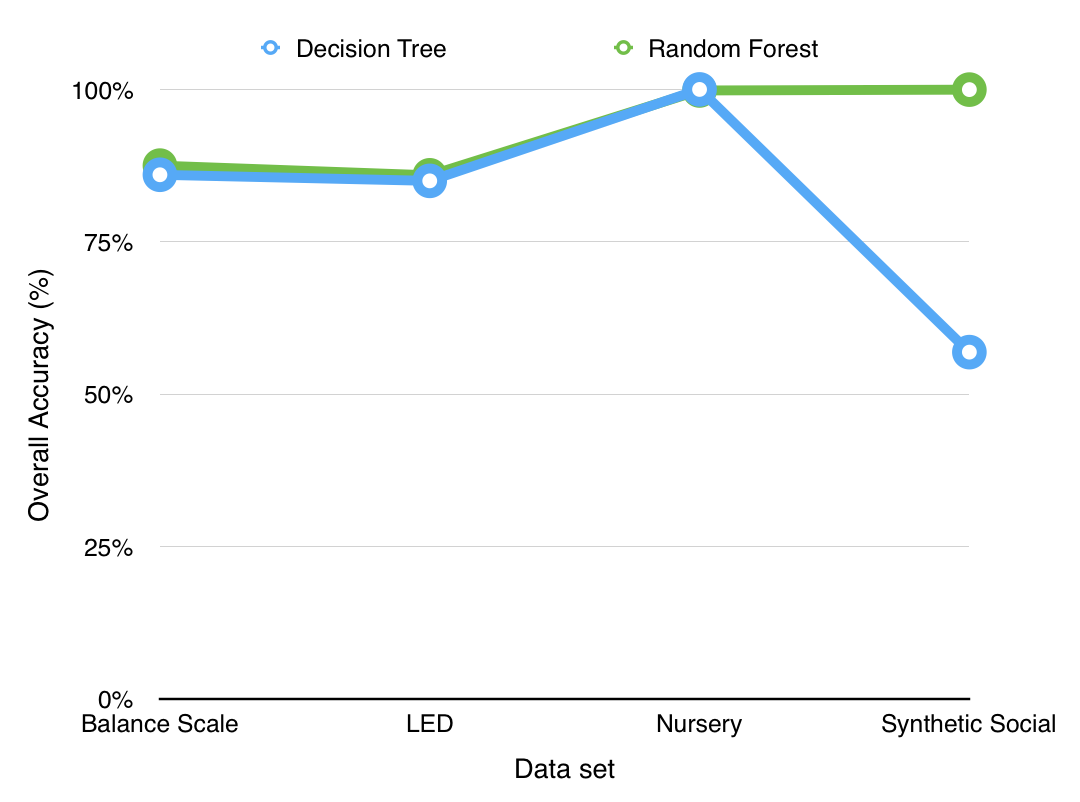
\includegraphics[scale=0.7]{overall-train.png}
\captionof{figure}{Comparison of overall accuracy when evaluated in the training data set.}
\end{center}

\begin{center}
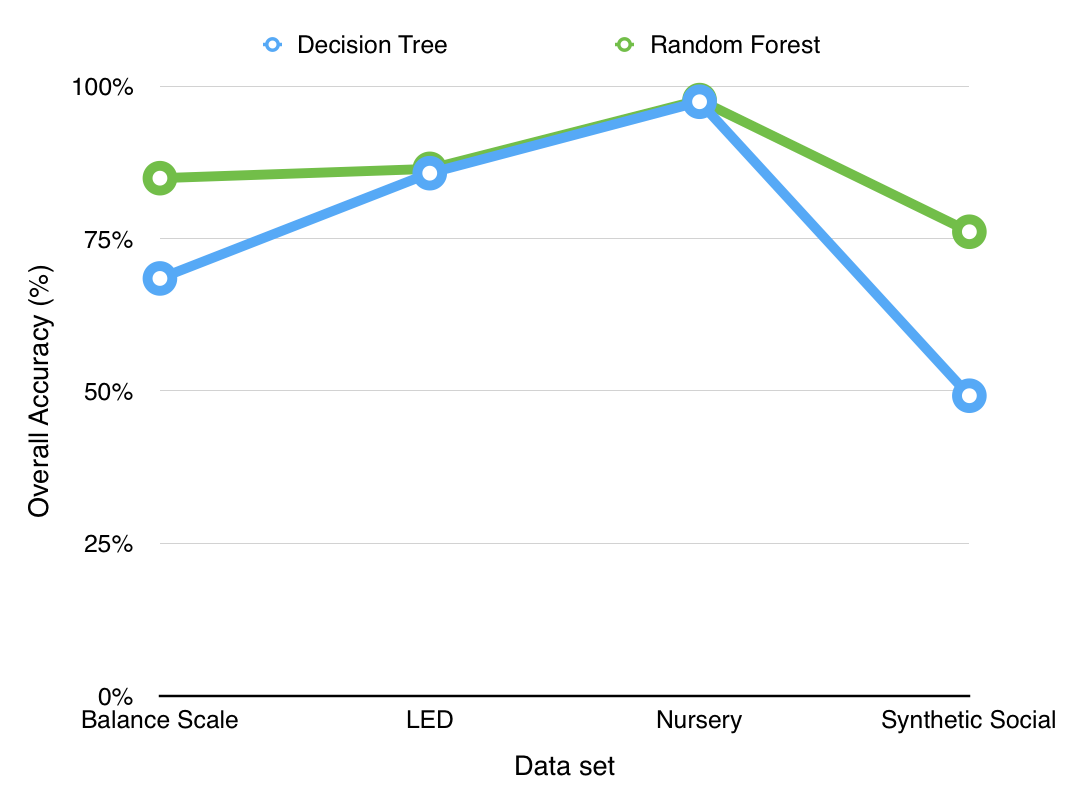
\includegraphics[scale=0.7]{overall-test.png}
\captionof{figure}{Comparison of overall accuracy when evaluated in the test data set.}
\end{center}

From the four data sets considered the Nursery data set did not improve considerable when using Random Forest. Another thing to note is that there are only two examples of the class 5 in this data set. The accuracy of the Random Forest oscilated between 97.4 and 97.7\% depending on whether those two elements ended up included in the data bag for some of the trees or not. Being higher when not included, which makes sense since there are no examples for the class in the test data so there is no chance of miss-classification. \\

Everything was executed in a MacBook Pro Mid 2015, 16GB RAM, i7 Processor and validated that would run under time constraints in the EWS Linux system (shared 128GB RAM, 24 cores). Even though the EWS system is more powerful the performance was better in my personal laptop. It seems to be a cap on the CPU time you can use simultaneously in EWS. When using the 24 cores I was only using like 15\% on each but when I changed to using only 5 cores they were all performed at 95\%. \\

\subsection*{Balance Scale Data set}

\subsection*{LED Data set}

\subsection*{Nursery Data set}
Although the results for Random Forest show an slight improvement over the Decision Tree, there were some cases in which the overall accuracy was slightly below 97.43\%. The only logical explanation for this is that, because of the number of trees and data bagging, there were some branches that were noisy. \\

For this particular data set the improvement is so small that, in my opinion, does not justify the added performance cost.

\subsection*{Synthetic Social Data set}
For this particular data set the improvement given by Random Forest is considerable. The classifier went from \textbf{49.2\%} to \textbf{76.1\%}; that represents a \textbf{54\%} improvement!


\end{document}
